Диффузионные модели, также известные как модели с диффузией, представляют собой класс вероятностных моделей, используемых для генерации данных, включая изображения.
Основная идея диффузионных моделей состоит в том, чтобы последовательно преобразовывать начальное изображение, добавляя к нему случайный шум на каждом шаге. Это делается путем итеративного применения условных вероятностных моделей, которые моделируют распределение пикселей изображения. Этот процесс постепенно улучшает качество изображения, приближая его к реальным данным из обучающего набора.
Важным преимуществом диффузионных моделей является их способность генерировать высококачественные изображения без необходимости использования генеративно-состязательных сетей или других архитектур глубокого обучения. Кроме того, эти модели позволяют контролировать процесс генерации изображений, например, регулируя уровень шума или изменяя другие параметры.
Таким образом, диффузионные модели представляют собой эффективный и гибкий метод генерации изображений, который находит применение в различных областях, включая компьютерное зрение, графический дизайн и искусственный интеллект.


\begin{figure}[h]
    \centering
    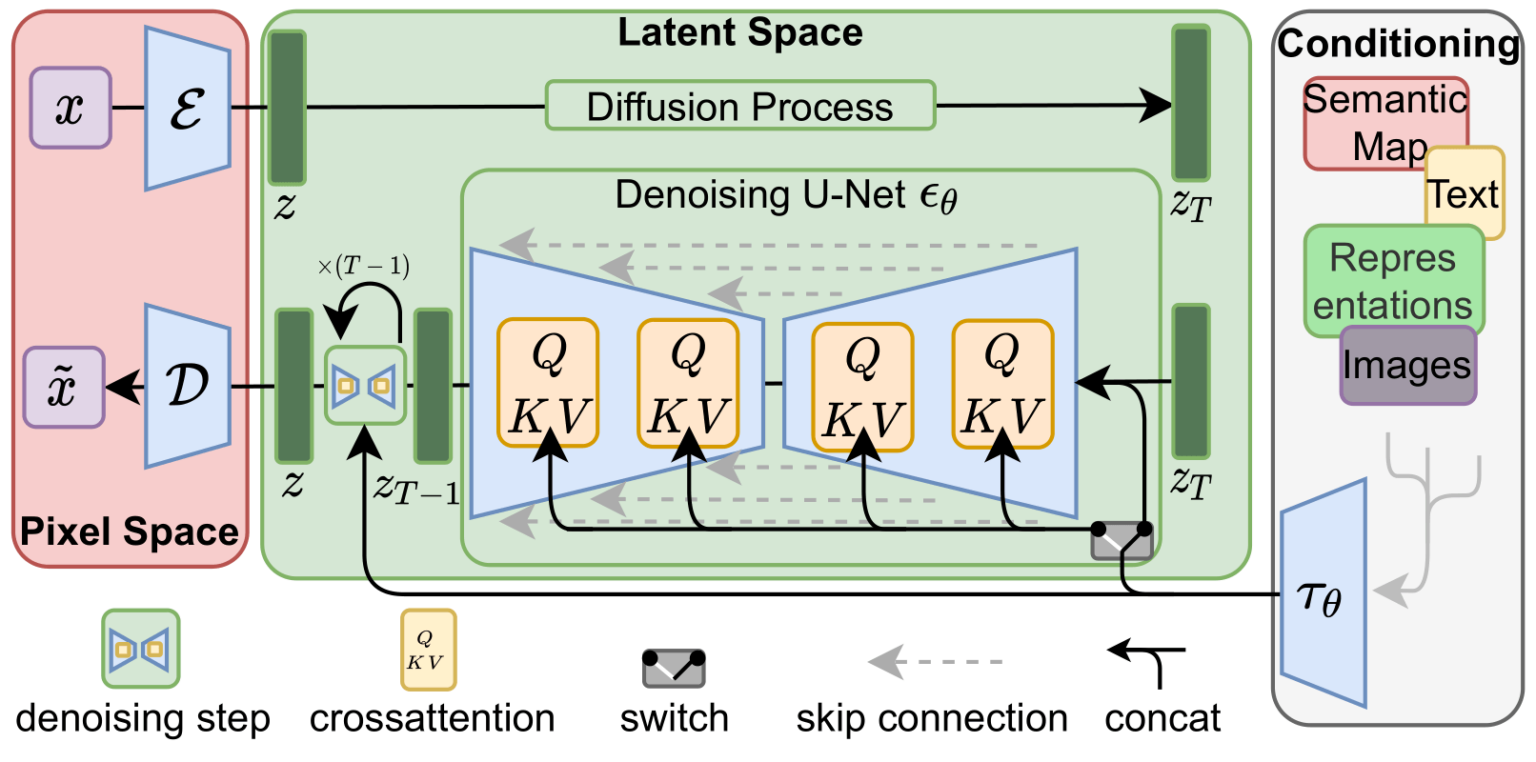
\includegraphics[width=0.5\textwidth]{assets/generation/stable_diffusion.png}
    \caption{Иллюстрация модели Stable Diffusion \cite{stablediffusion}}
    \label{sd_arch}
\end{figure}